\chapauthor{Гулякина Н.А.\\Козлова Е.И.\\Гракова Н.В.\\Оськин А.Ф.\\Головатый А.И.\\Самодумкин С.А.\\Ли В.}
\chapter{Автоматизация образовательной деятельности в рамках Экосистемы OSTIS}
\chapauthortoc{Гулякина Н.А.\\Козлова Е.И.\\Гракова Н.В.\\Оськин А.Ф.\\Головатый А.И.\\Самодумкин С.А.\\Ли В.}
\label{chapter_learning_systems}

\abstract{Аннотация к главе.}

\section{Общие принципы автоматизации образовательной деятельности с помощью ostis-систем}
\section{Автоматизация среднего образования с помощью ostis-систем}
\section{Автоматизация высшего образования с помощью ostis-систем}





\section{Семантические модели и средства контроля знаний пользователей в ostis-системах}

Данная подглава посвящена проблеме генерации тестовых вопросов и проверки ответов пользователей в интеллектуальных обучающих системах. В данной подглаве подробно представлен подход к автоматической генерации тестовых вопросов различных типов на основе базы знаний в интеллектуальных обучающих системах, разработанных с использованием Технологии OSTIS, и подход к реализации автоматической проверки ответов пользователей на основе различных семантических структур описанных знаний.

%Как деятельность прогресса и развития человеческого общества, образование внесло уникальный вклад в прогресс человеческой цивилизации. А со стремительным развитием науки и техники, оно играет всё более важную роль в современном обществе. В последние годы, с развитием современных информационных технологий, таких как искусственный интеллект, компьютерные исследователи начали работать над применением технологии искусственного интеллекта в сфере образования. Наиболее представительным продуктом, объединяющим технологии искусственного интеллекта и образования, являются интеллектуальные обучающие системы (ИОС).


Применение технологии искусственного интеллекта в сфере образования может не только повысить эффективность обучения учащихся, но и стать важным средством обеспечения справедливости образования. Особенно после вспышки COVID-19 в 2020 году была подчеркнута важность и актуальность разработки интеллектуальных обучающих систем (ИОС) [\scncite{Xu2009}]. По сравнению с традиционной мультимедийной обучающей системой (MОС), ИОС имеет следующие характеристики:

\begin{itemize}
	\item способен вести свободный человеко-машинный диалог;
	\item предоставление персонализированной педагогической услуги;
	\item автоматическое решение тестовых вопросов;
	\item автоматическая генерация тестовых вопросов;
	\item автоматическая проверка ответов пользователей;
	\item и т.д.
\end{itemize}

Среди перечисленных характеристик автоматическая генерация тестовых вопросов и автоматическая проверка ответов пользователей являются самыми основными и важными функциями ИОС. Они позволяют автоматизировать весь процесс от генерации тестовых вопросов и формирования экзаменационных билетов до автоматической проверки ответов пользователей и оценки экзаменационных билетов. Это может не только значительно повысить эффективность тестирования уровня знаний пользователей, но и снизить стоимость их обучения, при этом исключая человеческий фактор, чтобы максимально обеспечить справедливость процесса тестирования.

Хотя в последние годы с развитием семантической сети, обработки естественного языка (NLP) и других соответствующих технологий некоторыми научно-исследовательскими группами были предложены и разработаны подходы и системы для автоматической генерации тестовых вопросов и автоматической проверки ответов пользователей, эти подходы и системы имеют много недостатков, таких как:

\begin{itemize}
	\item только генерация простых объективных вопросов;
	\item большинство существующих подходов и систем проверки ответов поддерживает только проверку ответов пользователей на объективные вопросы;
	\item некоторые существующие подходы к проверке ответов пользователей на субъективные вопросы основаны на сопоставлении ключевых слов и статистике вероятности и не учитывают семантическое подобие между ответами;
	\item частично основанные на семантике подходы к проверке ответов пользователей на субъективные вопросы могут вычислять только подобие между ответами с простыми семантическими структурами;
	\item компоненты, разработанные с использованием существующих подходов к генерации тестовых вопросов и проверке ответов пользователей, могут быть использованы только в соответствующих системах;
	\item не поддерживается автоматизированная реализация всего процесса от генерации тестовых вопросов до проверки ответов пользователей [\scncite{Golenkov2014b}], [\scncite{Golenkov2019}], [\scncite{Li2020a}].
\end{itemize}

К типу вопросов с уникальным стандартным ответом относятся объективные вопросы, которые включают в себя: вопросы на выбор, вопросы суждения и вопросы на толкование определений. Субъективные вопросы не имеют уникальных ответов, а общие субъективные вопросы включают вопросы на доказательство, вопросы на толкование определений и решение задачи [\scncite{Li2021a}].

В связи с этим в данной подглаве представлен подход к автоматической генерации тестовых вопросов и автоматической проверке ответов пользователей в обучающих системах, разработанных с использованием Технологии OSTIS, и на основе предложенного подхода разработана универсальная подсистема для автоматической генерации тестовых вопросов и автоматической проверки ответов пользователей. Основной принцип автоматической генерации тестовых вопросов в данной работе заключается в том, чтобы сначала обобщить ряд стратегий генерации тестовых вопросов на основе структуры базы знаний ostis-систем и структуры представления знаний в ней, а затем использовать эти стратегии генерации тестовых вопросов для извлечения соответствующих семантических фрагментов из базы знаний и генерировать семантические модели, соответствующие тестовым вопросам [\scncite{Golenkov2014b}], [\scncite{IMS}]. Основной принцип проверки ответа на тестовый вопрос заключается в том, чтобы сначала вычислить подобие между семантическим графом стандартного ответа и семантическим графом ответа пользователя, а затем осуществить автоматическую проверку ответа пользователя на основе вычисленного подобия и стратегии оценки соответствующего тестового вопроса. Семантический граф представляет собой сеть, которая отображает семантические отношения между понятиями. В ostis-системах семантический граф строится с помощью SC-кода [\scncite{IMS}], [\scncite{Li2020a}]. Следует подчеркнуть, что семантический граф, соответствующий тестовому вопросу, и соответствующее ему описание на естественном языке преобразуются друг в друга с помощью естественно-языковых интерфейсов [\scncite{Qian2020a}]. Подход, предложенный в данной подглаве, должен решить следующие задачи:

\begin{itemize}
	\item автоматическая генерация ряда тестовых вопросов из базы знаний и сохранение их в соответствующих разделах базы знаний подсистемы;
	\item проектирование и построение баз знаний подсистем для хранения сгенерированных тестовых вопросов;
	\item извлечение соответствующих типов тестовых вопросов и составление экзаменационных билетов в соответствии с потребностями пользователей;
	\item вычисление подобия между семантическими графами ответов на объективные вопросы;
	\item вычисление подобия между семантическими графами ответов на вопросы на толкование определений;
	\item вычисление подобия между семантическими графами ответов на вопросы на доказательство и на решение задачи;
	\item автоматическая проверка ответов на тестовые вопросы и автоматическая оценка экзаменационных билетов на основе вычисленного подобия и стратегии оценки соответствующих тестовых вопросов.
\end{itemize}

Следует подчеркнуть, что предлагаемый в данной подглаве подход не опирается на какой-либо естественный язык, но для того, чтобы объяснить принцип работы предлагаемого подхода, подобранные в данной подглаве семантические фрагменты и иллюстрации представлены на русском языке. Среди них ostis-система по дискретной математике и ostis-система по евклидовой геометрии будут использоваться в качестве демонстрационных систем для подсистемы, разработанной с использованием предлагаемого подхода.

\subsection{Существующие научно-исследовательские результаты и проблемы}

\subsubsection{Автоматическая генерация тестовых вопросов}

Подход к автоматической генерации тестовых вопросов в основном изучает, как использовать электронные документы, корпуса текстов и базы знаний для быстрой и гибкой автоматической генерации тестовых вопросов. Благодаря тому, что знания в базе знаний представляют собой высокоструктурированные знания, прошедшие фильтрацию, и с развитием семантических сетей, использование базы знаний для автоматической генерации тестовых вопросов стало важнейшим направлением исследований в области автоматической генерации тестовых вопросов [\scncite{Xu2009}], [\scncite{Mousavinasab2018}], [\scncite{SinghBhatia2013}]. Некоторые результаты исследований приведены ниже:

\begin{itemize}
	\item подход к использованию классов, экземпляров, атрибутов и отношений между ними в онтологии OWL для генерации вопросов на выбор представлен в работе [\scncite{Papasalouros2008}]. OWL представляет собой язык описания онтологий для семантической сети. Онтология – это вид знаний, каждое из которых является спецификацией соответствующей предметной области, ориентированной на описание свойств и взаимосвязей понятий, входящих в состав указанной предметной области; 
	\item подход к автоматической генерации объективных вопросов с использованием онтологии, созданной Protégé [\scncite{Protege2016}], представлен в работе [\scncite{Li2012}].
\end{itemize}

Эти подходы в основном имеют следующие проблемы:

\begin{itemize}
	\item подход к использованию электронных документов для автоматической генерации тестовых вопросов требует большого количества шаблонов предложений;
	\item создание корпуса текстов требует больших человеческих ресурсов для сбора и обработки различных знаний;
	\item существующие подходы могут быть использованы только в соответствующих системах и не являются совместимыми;
	\item существующие подходы позволяют генерировать только простые объективные вопросы.
\end{itemize}

\subsubsection{Автоматическая проверка ответов пользователей}

Автоматическая проверка ответов пользователей делится на проверку ответов на объективные вопросы и проверку ответов на субъективные вопросы. Основной принцип проверки ответов на объективные вопросы относительно прост, то есть достаточно определить, совпадает ли строка стандартного ответа и строка ответа пользователя. Ответы на субъективные вопросы обычно не являются уникальными, поэтому основной принцип проверки ответов на субъективные вопросы заключается в вычислении подобия между стандартным ответом и ответом пользователя, а затем в осуществлении автоматической проверки ответов пользователя на основе вычисленного подобия и стратегии оценки соответствующих тестовых вопросов. Чем больше похожи стандартный ответ и ответ пользователя, тем выше подобие между ними [\scncite{Wan2019}], [\scncite{Lix2009}], [\scncite{Wan2019a}]. Проверка ответов на субъективные вопросы делится на следующие категории в соответствии с подходом, используемым для вычисления подобия:

\begin{itemize}
	\item На основе ключевых словосочетаний
	
	Этот тип подхода позволяет сначала разделить предложения на ключевые словосочетания, а затем вычислить подобие между ними в соответствии с отношениями совпадения ключевых словосочетаний между предложениями. Представительные подходы включают:
	
	\begin{itemize}
		\item N-gram similarity
		\item Jaccard similarity
	\end{itemize}
	
	\item На основе модели векторного пространства (VSM)
	
	Основной принцип VSM заключается в использовании традиционных алгоритмов машинного обучения для того, чтобы сначала преобразовать предложения в векторные представления, а затем вычислить подобие между ними [\scncite{Shahmirzadi2019}]. Представительные подходы включают:
	
	\begin{itemize}
		\item TF-IDF
		\item Word2vec
		\item Doc2Vec
	\end{itemize}
	
	\item На основе глубокого обучения
	
	Этот тип подхода позволяет использовать модели нейронных сетей для вычисления подобия между предложениями [\scncite{Ji2022}]. Представительные модели нейронных сетей включают:
	
	\begin{itemize}
		\item Tree-LSTM
		\item Transformer
		\item BERT
	\end{itemize}
	
	\item На основе семантического графа
	
	Основной принцип вычисления подобия между ответами с использованием данного типа подхода заключается в том, чтобы сначала преобразовать ответы (т.е. предложения или короткие тексты) в представление семантического графа с помощью инструментов обработки естественного языка (например, синтаксические деревья зависимостей и естественно-языковые интерфейсы), а затем вычислить подобие между семантическими графами (т.е. подобие между ответами). В ИОС различная информация хранится в виде семантических графов, поэтому можно рассмотреть возможность вычисления подобия между любыми двумя семантическими графами в базе знаний, опираясь на принципы работы данного типа подхода. Основным преимуществом этого типа подхода является вычисление подобия между ответами на основе семантики. Одним из наиболее представительных подходов является SPICE (Semantic Propositional Image Caption Evaluation) [\scncite{Anderson2016}]. 
	
	Подход SPICE используется для вычисления подобия между автоматически сгенерированными подписями к рисункам (подписи-кандидаты) и подписями к рисункам, помеченными вручную (подписи-образцы). Данный подход позволяет вычислить подобие между подписями путем сопоставления одного и того же числа кортежей между семантическими кортежами подписи-кандидатов и семантическими кортежами подписи-образцов.
	
\end{itemize}

Эти подходы в основном имеют следующие недостатки:

\begin{itemize}
	\item подход, основанный на ключевых словосочетаниях, не учитывает порядок между словами в предложении;
	\item подход на основе VSM приводит к генерации высокоразмерных разреженных матриц, что увеличивает сложность алгоритма;
	\item подходы на основе семантических графов, поддерживающие только описание простых семантических структур;
	\item эти подходы не позволяют определить, являются ли предложения логически эквивалентными друг другу;
	\item эти подходы зависят от соответствующего естественного языка.
\end{itemize}

Поэтому на основе существующих подходов к автоматической генерации тестовых вопросов с использованием баз знаний, подходов к вычислению подобия между ответами с использованием семантических графов и Технологии OSTIS в данной подглаве предлагается подход к автоматической генерации тестовых вопросов и автоматической проверке ответов пользователей с использованием семантики.

\subsection{Предложенный подход и семантические модели пользователей}

Основной задачей данной подглавы является детализация подхода к автоматической генерации тестовых вопросов и автоматической проверке ответов пользователей в ostis-системах и разработка универсальной подсистемы на основе этого подхода. Где универсальность подсистемы означает, что подсистема может быть легко перенесена между различными ostis-системами. Предлагаемый подход можно разделить на две части в соответствии с реализуемыми функциями, т.е. автоматическая генерация тестовых вопросов и автоматическая проверка ответов пользователей [\scncite{Li2021a}]. Поэтому мы представим процесс реализации этих двух частей отдельно.

\subsubsection{Предлагаемый подход к автоматической генерации тестовых вопросов}

Основной принцип автоматической генерации различных типов тестовых вопросов (включая объективные вопросы и субъективные вопросы) в ostis-системах заключается в том, чтобы сначала извлечь соответствующие семантические фрагменты из базы знаний, используя ряд стратегий генерации тестовых вопросов, обобщённых на основе подхода представления знаний и структуры описания знаний в рамках Технологии OSTIS, затем добавить к извлечённым семантическим фрагментам информацию об описании тестового вопроса и, наконец, сохранить семантические фрагменты, описывающие полные тестовые вопросы, в соответствующем разделе подсистемы [\scncite{Golenkov2014b}]. Когда необходимо сформировать экзаменационные билеты, подсистема позволяет извлечь из базы знаний подсистемы несколько соответствующих тестовых вопросов в соответствии с параметрами, введёнными пользователем, и объединить их в экзаменационные билеты. Тестовые вопросы и экзаменационные билеты в виде семантических графов преобразуются в описания на естественном языке с помощью естественно-языковых интерфейсов. В работе [\scncite{Li2020a}] мы подробно рассмотрели некоторые стратегии, используемые для автоматической генерации тестовых вопросов в ostis-системах, далее мы выберем только некоторые из стратегий генерации тестовых вопросов для представления.

\begin{itemize}
	\item Стратегия генерации тестовых вопросов на основе класса
	
	Этот тип стратегии генерации тестовых вопросов используется для автоматической генерации объективных вопросов, основанных на различных отношениях между классами. Далее она делится на:
	
	\begin{itemize}
		\item На основе отношения "включение*"
		
		Отношение включения является одним из наиболее часто используемых отношений в базе знаний ostis-систем, которое удовлетворяется между многими классами (включая подклассы), поэтому отношение включения между классами может быть использовано для генерации объективных вопросов. Форма выражения в теории множеств отношения включения между классами выглядит следующим образом: $S_{i}\subseteq  C $, ($S$ – подкласс, $i$ – номер подкласса, $C$ – родительский класс). Ниже показан семантический фрагмент в базе знаний, который удовлетворяет отношению включения в SCn-коде [\scncite{Golenkov2014b}], [\scncite{IMS}]: 
		
		\scnheader{бинарное дерево}
		\scnrelto{включение}{ориентированное дерево}
		\begin{scnrelfromlist}{включение} 
			\scnitem{братское дерево}
			\scnitem{дерево решений}
			\scnitem{бинарное дерево сортировки}
		\end{scnrelfromlist}
		
		В качестве примера вопроса на выбор, сгенерированного с использованием этого семантического фрагмента на основе стратегии отношений включения, ниже показана его форма на естественном языке:
		
		<<Частным случаем бинарного дерева не является (\ )?>>
		
		A. дерево решений   \quad C. ориентированное дерево \\
		B. братское дерево  \quad D. бинарное дерево сортировки
		
		Пример семантической модели данного тестового вопроса приведён на рисунке (\textit{\nameref{fig:mc_example}}) в SCg-коде.
		
		Аналогичным образом, используя эту стратегию, можно генерировать другие типы объективных вопросов;
		
		\item На основе отношения "разбиение*"
		
		Отношение разбиения – это квазибинарное ориентированное отношение, областью определения которого является семейство всевозможных множеств. В  результате разбиения множества получается множество попарно непересекающихся множеств, объединение которых есть исходное множество. Отношение разбиения также является важным отношением в базе знаний, поэтому семантические фрагменты в базе знаний, удовлетворяющие этому отношению, могут быть использованы для генерации объективных вопросов. На языке теории множеств отношение разбиения между классами описывается следующим образом: $S_{i_{1}}\cup  S_{i_{2}}\cdots S_{i_{m}} \cup S_{i_{n}} = S_{j_{1}}\cup  S_{j_{2}}\cdots S_{j_{m}} \cup S_{j_{n}}= \cdots = U$, ($n>1$, $S_{j_{m}} \cap S_{j_{n}} = \oslash$). Ниже приведён семантический фрагмент в базе знаний, удовлетворяющий отношению "разбиение*"\ в SCn-коде:
		
		\scnheader{граф}
		\scnrelfrom{включение}{полуэйлеров граф}
		\begin{scnreltoset}{разбиение}
			\scnitem{невзвешенный граф}
			\scnitem{взвешенный граф}
		\end{scnreltoset}
		\begin{scnreltoset}{разбиение}
			\scnitem{непланарный граф}
			\scnitem{планарный граф}
		\end{scnreltoset}
		\begin{scnreltoset}{разбиение}
			\scnitem{несвязный граф}
			\scnitem{связный граф}
		\end{scnreltoset}
		
		\begin{figure}[H]
			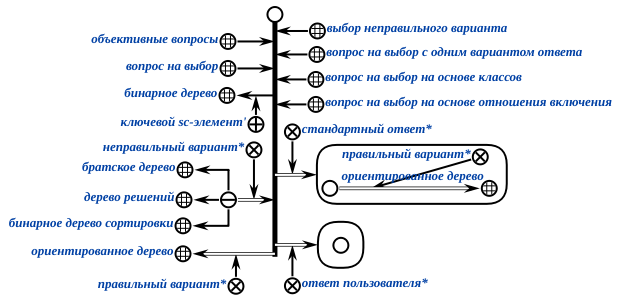
\includegraphics[scale=1]{author/part7/figures/MC_question_example.png}
			\caption{Пример семантической модели вопроса на выбор}
			\label{fig:mc_example}
		\end{figure}
		
		\item На основе отношения "строгое включение*"
		
		Отношение строгого включения является особой формой отношения включения ($S_{i}\subset  C $, ($i\ge 1$)). Использование отношения строгого включения для автоматической генерации объективных вопросов аналогично использованию отношения включения. Ниже приведён семантический фрагмент в базе знаний, удовлетворяющий отношению "строгое включение*"\ в SCn-коде:
		
		\scnheader{Предметная область множеств}
		
		\begin{scnhaselementrolelist}{немаксимальный класс объектов исследования}
			\scnitem{счётное множество}
			\scnitem{ориентированное множество}
			\scnitem{конечное множество} 
			\begin{scnrelfromlist}{включение} 
				\scnitem{пара}
				\scnitem{тройка}
			\end{scnrelfromlist}
		\end{scnhaselementrolelist}
		
	\end{itemize}
	
\end{itemize}	

Другие стратегии, используемые для генерации объективных вопросов, также включают:
\begin{itemize}
	\item Стратегия генерации тестовых вопросов на основе элементов;
	\item Стратегия генерации тестовых вопросов на основе идентификаторов;
	\item Стратегия генерации тестовых вопросов на основе аксиом; 
	\item Стратегия генерации тестовых вопросов на основе атрибутов отношений;
	\item Стратегия генерации тестовых вопросов на основе примеров изображений.
\end{itemize}

Конкретный процесс генерации объективных вопросов с использованием перечисленных выше стратегий подробно представлен в работе [\scncite{Li2020a}].

Процесс генерации субъективных вопросов с использованием стратегии генерации субъективных вопросов выглядит следующим образом:

\begin{itemize}
	\item поиск в базе знаний семантических фрагментов, описывающих субъективные вопросы с использованием логических правил (т.е. шаблоны, построенные с использованием SC-кода);
	\item хранение найденных семантических фрагментов в соответствующем разделе базы знаний подсистемы;
	\item использование ручных подходов или автоматических подходов (например, с помощью естественно-языковых интерфейсов) для описания определения, процесса доказательства или процесса решения соответствующего тестового вопроса в соответствии с правилами представления знаний (т.е. стандартные ответы на субъективные вопросы). Среди них стандартные ответы на субъективные вопросы представлены с помощью SCg-кода или SCL-кода [\scncite{Golenkov2014b}], [\scncite{IMS}]. 
	
\end{itemize}

Пример семантической модели субъективного вопроса показан на рисунке (\textit{\nameref{fig:DI_example}}) в SCg-коде.

\begin{figure}[H]
	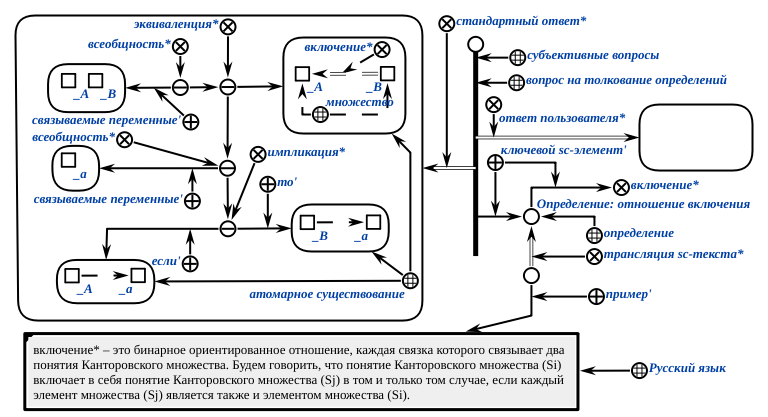
\includegraphics[scale=0.8]{author/part7/figures/DI_question_example.png}
	\caption{Семантическая модель определения отношения включения}
	\label{fig:DI_example}
\end{figure}

На рисунке (\textit{\nameref{fig:DI_example}}) описано определение отношения включения ($\forall A\forall B((A\subseteq B)\Longleftrightarrow (\forall a(a\in A\rightarrow a\in B))$).

Использование этих стратегий генерации тестовых вопросов, описанных выше, позволяет генерировать различные типы тестовых вопросов автоматически из базы знаний. Эти автоматически сгенерированные тестовые вопросы хранятся в базе знаний подсистемы в соответствии с их типом и соответствующей стратегией генерации тестовых вопросов. Такой тип хранения позволяет быстро и динамично генерировать экзаменационные билеты в соответствии с потребностями пользователя. В следующем подразделе мы подробно опишем построение базы знаний подсистемы и способ хранения в ней тестовых вопросов. Предлагаемый подход к генерации тестовых вопросов имеет следующие преимущества:

\begin{itemize}
	\item Технология OSTIS поддерживает унифицированные подходы к представлению знаний и структуры описания знаний, поэтому предложенный подход к генерации тестовых вопросов может быть использован в различных ostis-системах;
	\item сгенерированные тестовые вопросы описываются с помощью SC-кода, поэтому они не опираются на какой-либо естественный язык;
	\item используя предложенный подход к генерации тестовых вопросов, можно генерировать не только объективные вопросы, но и субъективные вопросы.
\end{itemize}

\subsubsection{Предложенный подход к автоматической проверке ответов пользователей}

В ostis-системах тестовые вопросы хранятся в базе знаний в виде семантических графов, поэтому наиболее важным этапом проверки ответов пользователей является вычисление подобия между семантическим графом стандартного ответа и семантическим графом ответа пользователя, и когда подобие получено и объединено со стратегией оценки соответствующих тестовых вопросов, правильность и полнота ответов пользователей могут быть проверены [\scncite{Golenkov2019}], [\scncite{Li2021a}].

В соответствии с типом тестовых вопросов проверка ответов пользователей классифицируется как:

\begin{itemize}
	\item проверка ответов на объективные вопросы;
	\item проверка ответов на субъективные вопросы.
\end{itemize}

Хотя наиболее важным этапом проверки ответов является вычисление подобия между семантическими графами ответов, типы знаний (фактические знания и логические знания) и структуры знаний, используемые для описания различных типов тестовых вопросов, не одинаковы, поэтому подходы к вычислению подобия между семантическими графами ответов на различные типы тестовых вопросов различны. Фактические знания относятся к знаниям, которые не содержат типов переменных, и этот тип знаний выражает факты. Логические знания обычно содержат переменные, и между ними существуют логические отношения. В ostis-системах SCL-код используется для описания логических знаний. В ostis-системах объективные вопросы, вопросы на доказательство и решение задачи описываются с использованием фактических знаний, а вопросы на толкование определений описываются с использованием фактических и логических знаний вместе.

\subsubsection{Проверка ответов на объективные вопросы}

Семантические графы, используемые для описания объективных типов тестовых вопросов и ответов на них в базе знаний, имеют одинаковую семантическую структуру, поэтому подобие между ответами на такие типы тестовых вопросов может быть вычислено с использованием того же подхода. Поскольку ответы пользователей на естественном языке на объективные вопросы уже согласованы с существующими знаниями в базе знаний, когда они преобразуются в семантические графы с помощью естественно-языкового интерфейса, то есть элементы, представляющие одну и ту же семантику в базе знаний, имеют один и тот же основной идентификатор [\scncite{Qian2020a}]. Поэтому при вычислении подобия между семантическими графами ответов на объективные вопросы нет необходимости учитывать различия между понятиями на уровне естественного языка, то есть подобие между ответами вычисляется на основе семантических структур. Для проверки ответов пользователей на объективные вопросы необходимо решить следующие задачи:

\begin{itemize}
	\item вычисление подобия между семантическими графами ответов на объективные вопросы;
	\item определение того, существует ли логическая эквивалентность между семантическими графами ответов на объективные вопросы (семантическими графами ответов, описанными на основе фактических знаний);
	\item использование вычисленного подобия и стратегий оценки объективных вопросов для проверки правильности и полноты ответов пользователей и подсчета баллов за ответы пользователей.
\end{itemize}

Логическая эквивалентность между семантическими графами в ostis-системах делится на два типа:

\begin{itemize}
	\item логическая эквивалентность между семантическими графами, описанными на основе логических формул;
	\item логическая эквивалентность между семантическими графами, описанными на основе различных систем понятий (различных по структуре семантических графов). Этот тип логической эквивалентности далее классифицируется в зависимости от типа знания:
	
	\begin{itemize}
		\item логическая эквивалентность между семантическими графами, описанными на основе фактических знаний;
		\item логическая эквивалентность между семантическими графами, описанными на основе логических знаний.
	\end{itemize}
	
\end{itemize}

Основной принцип вычисления подобия между семантическими графами ответов на объективные вопросы показан ниже:

\begin{itemize}
	\item декомпозиция семантического графа стандартного ответа ($s$) и семантического графа ответа пользователя ($u$) на подструктуры в соответствии с правилами представления фактических знаний;
	\item использование формул (\ref{formula_7_5_1}), (\ref{formula_7_5_2}) и (\ref{formula_7_5_3}) для вычисления точности ($P_{sc}$), полноты ($R_{sc}$) и подобия ($F_{sc}$) между семантическими графами.  
\end{itemize}

\begin{equation}    
	P_s{_c}(u,s) = \frac{|T_s{_c}(u)\otimes T_s{_c}(s)|}{|T_s{_c}(u)|}  
	\label{formula_7_5_1} 
\end{equation}  

\begin{equation}    
	R_s{_c}(u,s) = \frac{|T_s{_c}(u)\otimes T_s{_c}(s)|}{|T_s{_c}(s)|}  
	\label{formula_7_5_2} 
\end{equation}  

\begin{equation}    
	F_s{_c}(u,s) = \frac{2\cdot P_s{_c}(u,s)\cdot R_s{_c}(u,s)}{P_s{_c}(u,s) + R_s{_c}(u,s)}  
	\label{formula_7_5_3} 
\end{equation}

где:

\begin{itemize}
	\item ($\otimes$) --- бинарный оператор сопоставления;
	
	\item множество $T_{sc}(s)$ --- все разложенные подструктуры стандартного ответа $s$;
	
	\item множество $T_{sc}(u)$ --- все разложенные подструктуры стандартного ответа $u$;
\end{itemize}

Поскольку подсистема также должна позволять вычислять подобие между любыми двумя семантическими графами в базе знаний, вычисленное подобие может быть использовано в будущем для проверки ответов пользователя на новые типы тестовых вопросов и для решения других задач, таких как слияние знаний. В базе знаний содержится большое количество семантических графов, имеющих схожую структуру с семантическими графами ответов на объективные вопросы, т.е. семантических графов, описанных с помощью фактических знаний, поэтому подход, используемый для вычисления подобия между ответами на объективные вопросы, также может быть использован для вычисления подобия между семантическими графами, описанными с помощью фактических знаний. Поскольку семантический граф ответов на объективные вопросы и семантический граф, описанный с использованием фактических знаний, имеют схожую семантическую структуру, далее они будут единообразно именоваться семантическим графом ответов на объективные вопросы. Но семантические графы этого типа обычно имеют семантические графы, логически эквивалентные им, например, определение симметричной разности может быть выражено в этих двух формах:

\begin{itemize}
	\item $C= \left ( A\setminus B \right ) \cup \left ( B \setminus A \right )$;
	\item $C= A\bigtriangleup B$.
\end{itemize}

Поэтому, если вычисленное подобие между семантическими графами не равно 1, необходимо также определить, удовлетворяется ли между ними логическая эквивалентность. Поэтому в данной подглаве представлен подход к определению логической эквивалентности между семантическими графами, описанными на основе фактических знаний.

Процесс определения логической эквивалентности между семантическими графами такого типа показан ниже:

\begin{enumerate}
	\item найдены все sc-узлы в семантическом графе стандартного ответа и все sc-узлы в семантическом графе ответа пользователя соответственно. Затем проверяется, существует ли пара sc-узлов между sc-узлами стандартного ответа и sc-узлами ответа пользователя, и ее два sc-узла соответственно включены в шаблон, связанный с использованием отношения "эквиваленция*". Если такая пара sc-узлов существует, выполняется следующий шаг. Пример пары шаблонов показан на рисунке (\textit{\nameref{fig:ET_example}}) в SCg-коде;
	\begin{figure}[H]
		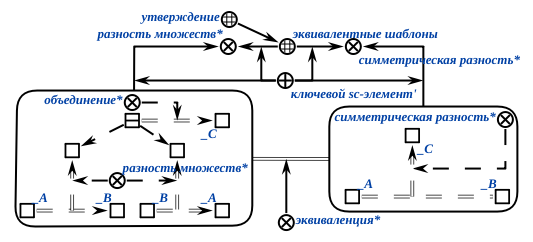
\includegraphics[scale=1]{author/part7/figures/equivalent_template_example.png}
		\caption{Пара шаблонов, удовлетворяющих логической эквивалентности}
		\label{fig:ET_example}
	\end{figure}
	
	\item использование двух шаблонов для поиска всех соответствующих семантических фрагментов в базе знаний и проверка наличия двух семантических фрагментов в этих найденных семантических фрагментах, которые соответственно включены в стандартный ответ и ответ пользователя. Если существуют такие два семантических фрагмента (соответствие различным шаблонам), выполняется следующий шаг;
	
	\item итеративно проходятся разложенные подструктуры стандартного ответа и разложенные подструктуры ответа пользователя, и каждая подструктура сравнивается с соответствующим семантическим фрагментом, найденным на шаге 2, если каждый sc-элемент в подструктуре содержится в соответствующем семантическом фрагменте, подструктура удаляется;
	
	\item использование формул (\ref{formula_7_5_1}), (\ref{formula_7_5_2}) и (\ref{formula_7_5_3}) для вычисления подобия между семантическими графами в соответствии с остальными подструктурами. Если подобие равно 1, то два семантических графа полностью совпадают.
	
\end{enumerate}

Пример определения логической эквивалентности семантических графов приведён на рисунке (\textit{\nameref{fig:LE_example}}) в SCg-коде. 

Когда получено подобие ответов, можно проверить правильность и полноту ответов пользователей на объективные вопросы, объединив их со стратегией оценки объективных вопросов. Стратегия оценки объективных вопросов показана ниже:

\begin{itemize}
	\item если для текущего тестового вопроса существует только один правильный вариант, только если стандартный ответ и ответ пользователя точно совпадают, ответ пользователя считается правильным, и пользователь получает максимальный балл ($Max_{score}$);
	
	\item если текущий вопрос имеет несколько правильных вариантов (например, вопросы на выбор с несколькими вариантами ответов и часть вопросов на заполнение пробелов):
	
	\begin{itemize}
		\item до тех пор, пока ответ пользователя содержит неправильный вариант, ответ пользователя считается неправильным и оценка пользователя равна 0;
		
		\item если все варианты в ответе пользователя правильные, но количество правильных вариантов меньше, чем количество правильных вариантов в стандартном ответе, ответ пользователя считается правильным, но неполным. В это время оценка ответа пользователя равна $R_{sc}*Max_{score}$;
		
		\item если все варианты стандартного ответа точно совпадают со всеми вариантами ответа пользователя, то ответ пользователя точно правильный, а оценка пользователя равна $Max_{score}$. 	
		
	\end{itemize}
	
\end{itemize}

\begin{figure}[H]
	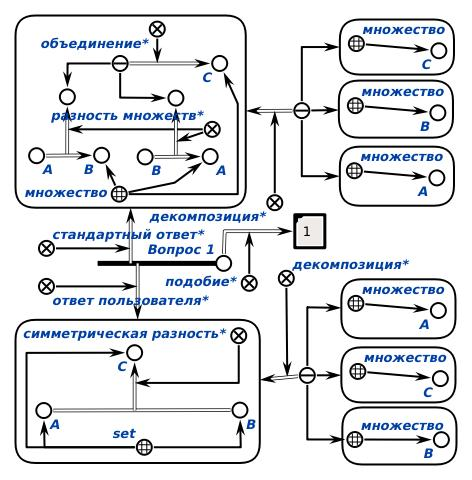
\includegraphics[scale=0.7]{author/part7/figures/logical_equivalence_example.jpg}
	\caption{Пример суждения логической эквивалентности семантических графов, описанных на основе фактических знаний}
	\label{fig:LE_example}
\end{figure}

Пример проверки ответов на конкретный объективный вопрос показан на рисунке (\textit{\nameref{fig:AV_example}}) в SCg-коде.

\subsubsection{Проверка ответов на субъективные вопросы}

Наиболее важным этапом проверки ответов на субъективные вопросы также является вычисление подобия между семантическими графами ответов, однако типы знаний и структуры знаний, используемые для описания различных типов субъективных вопросов и ответов на них, в ostis-системах не одинаковы. Таким образом, подход к вычислению подобия между семантическими графами ответов на субъективные вопросы далее делится на:

\begin{itemize}
	\item подход к вычислению подобия между ответами на вопросы на толкование определений;
	\item подход к вычислению подобия между ответами на вопросы на доказательство и на решение задачи.
\end{itemize} 
~\\
\textbf{Вычисление подобия между ответами на вопросы на толкование определений} 

~\\
Ответы на вопросы на толкование определений в ostis-системах описываются в виде логических формул с использованием фактических знаний и логических знаний (SCL-кода). Логическая формула является мощным инструментом для формального представления знаний в рамках Технологии OSTIS, которая расширяется на основе формул логики предикатов первого порядка и наследует все операционные свойства формул логики предикатов первого порядка [\scncite{IMS}]. Следует подчеркнуть, что при вычислении подобия между ответами на вопросы на толкование определений, фактические знания в семантических графах ответов пользователей были согласованы с существующими знаниями в базе знаний (с использованием естественно-языковых интерфейсов) [\scncite{Qian2020a}]. Для вычисления подобия между семантическими графами ответов на вопросы на толкование определений необходимо решить следующие задачи [\scncite{Fujiwara2021}]:

\begin{itemize}
	\item автоматический выбор потенциального эквивалентного стандартного ответа;
	\item установление отношений отображения потенциальных эквивалентных пар переменных sc-узлов между семантическими графами ответов;
	\item вычисление подобия между семантическими графами;
	\item если подобие между семантическими графами не равно 1, то их также необходимо отдельно преобразовать в представление префиксной нормальной формы (ПНФ/PNF), а затем снова вычислить подобие между ними.
\end{itemize}

\begin{figure}[H]
	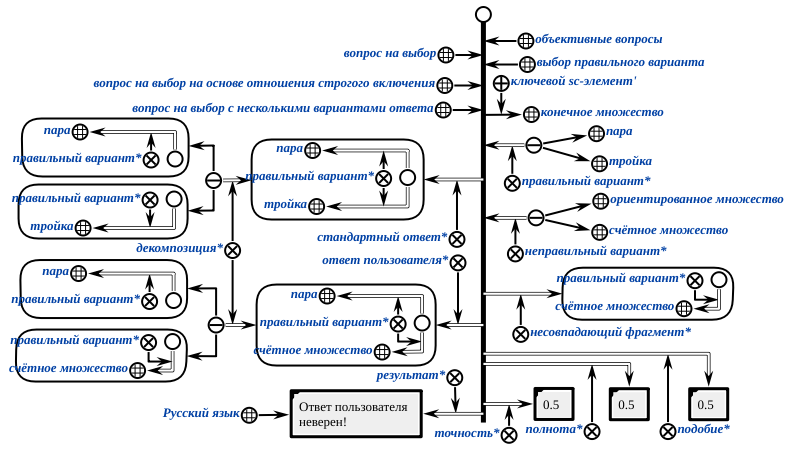
\includegraphics[scale=0.7]{author/part7/figures/answer_verification_example.png}
	\caption{Пример автоматической оценки вопроса на выбор с несколькими вариантами ответа}
	\label{fig:AV_example}
\end{figure}

Некоторые вопросы на толкование определений иногда имеют несколько стандартных ответов, но логические формулы, используемые для их формального представления, не являются логически эквивалентными (описываются в соответствии с различными системами понятий). Например, определение отношения эквивалентности:

\begin{itemize}
	\item в математике отношение эквивалентности является бинарным отношением, которое является рефлексивным, симметричным и транзитивным;
	\item для любого бинарного отношения, если оно является толерантным отношением и транзитивным, то оно является отношением эквивалентности.
\end{itemize}

Поэтому при вычислении подобия между ответами необходимо заранее отфильтровать стандартный ответ, который наилучшим образом соответствует ответу пользователя, из нескольких возможных стандартных ответов. Поэтому в данной подглаве предлагается подход к фильтрации стандартного ответа, который наилучшим образом соответствует ответу пользователя в соответствии с подобием предикатов между ответами. Принцип работы этого подхода показан ниже:

\begin{itemize}
	\item нахождение всех предикатов в каждом ответе (неповторяющихся предикатов);
	\item вычисление подобия предикатов между ответом пользователя и каждым стандартным ответом с использованием формул (\ref{formula_7_5_1}), (\ref{formula_7_5_2}) и (\ref{formula_7_5_3}); 
	\item стандартный ответ, который наиболее похож (максимальное подобие) на ответ пользователя, выбирается в качестве окончательного стандартного ответа.
\end{itemize}

Поскольку семантические графы, используемые для описания ответов на вопросы на толкование определений, построены на основе логических формул, в семантические графы включены переменные sc-узлов (эквивалентные связанным переменным в формуле логики предикатов). Для того чтобы рассчитать подобие между семантическими графами, наиболее важным шагом является установление отношений отображения потенциальных эквивалентных пар переменных sc-узлов между семантическими графами. Поэтому на основе существующих методов отображения онтологий и систем отображения онтологий (например, ASMOW, RiMOM и др.) в данной подглаве предлагается подход к установлению отношений отображения потенциальных эквивалентных пар переменных sc-узлов между семантическими графами в соответствии с семантическими структурами (различными sc-конструкциями) [\scncite{Zeng2021}], [\scncite{Sun2020}], [\scncite{Rujiang2011}].

В ostis-системах sc-конструкция, состоящая из sc-кортежа, sc-узла отношения, sc-узла ролевого отношения и sc-коннектора, используется для описания логических связок (такие как отрицание ($\lnot$) и импликация ($\to$), и т.д.) и кванторов (квантора всеобщности ($\forall$) и квантора существования ($\exists$)). Атомарная логическая формула (различные sc-конструкции) или несколько атомарных логических формул, удовлетворяющих отношению конъюнкции, содержатся в sc-структуре и связаны с соответствующим sc-кортежем, и эти sc-элементы вместе составляют семантический граф, используемый для представления ответа пользователя [\scncite{Golenkov2014b}], [\scncite{Rujiang2011}]. Все sc-кортежи и sc-коннекторы образуют дерево, которое полностью описывает логическую последовательность между связками и кванторами в логической формуле. Поскольку sc-структура, содержащая атомарную логическую формулу, связана с соответствующим sc-кортежем, пока определена позиция каждого sc-кортежа и sc-структуры в семантическом графе, можно определить позицию каждой переменной sc-узла в семантическом графе. В данной подглаве предлагается подход к нумерации каждого sc-кортежа и sc-структуры в семантическом графе в соответствии со стратегией поиска в глубину (DFS). Процесс работы данного подхода показан ниже:

\begin{itemize}
	\item начиная с корня древовидной структуры, состоящей из sc-кортежей, каждый узел sc-кортежа в дереве нумеруется по очереди в соответствии со стратегией DFS и приоритетом текущего sc-узла (например, приоритет sc-узла условия "если' "\ выше, чем приоритет sc-узла вывода "то' ") (последовательность нумерации начинается с 0);
	\item в соответствии с последовательностью нумерации sc-кортежей, каждый sc-кортеж в дереве обходится от малого к большому, а sc-структура, связанная с текущим sc-кортежем, нумеруется при обходе (последовательность нумерации начинается с 1).
\end{itemize}

При проверке ответа, если стандартный ответ и ответ пользователя точно равны, это означает, что атомарные логические формулы с одинаковой семантикой между ответами имеют одинаковое положение в семантическом графе (то есть, последовательность нумерации sc-структуры одинакова). Поэтому в данной подглаве отношения отображения потенциальных эквивалентных пар переменных sc-узлов будут устанавливаться на основе отношений соответствия sc-конструкций в одной и той же позиции между ответами. Процесс установления отношений отображения потенциальных эквивалентных пар переменных sc-узлов между ответами показан ниже:

\begin{enumerate}
	\item в соответствии с последовательностью нумерации sc-структур в семантическом графе, каждый раз, когда из стандартного ответа и ответа пользователя найдена пара sc-структур с одинаковым номером;
	\item в соответствии с порядком приоритета (от высокого к низкому) различных типов sc-конструкций, используемых для описания атомарной логической формулы, поочередно определяется, содержит ли текущая пара sc-структур одновременно данный тип sc-конструкции. Если этот тип sc-конструкции одновременно содержится в текущей паре sc-структур, то, в соответствии с отношением соответствия каждого sc-элемента между текущей sc-конструкцией в стандартном ответе и текущей sc-конструкцией в ответе пользователя, устанавливаются отношения отображения потенциальных эквивалентных пар переменных sc-узлов между текущими sc-конструкциями;
	\item повторять шаг 1 --- шаг 2, пока не будут установлены все отношения отображения между семантическими графами [\scncite{Li2021a}].
\end{enumerate}

На рисунке (\textit{\nameref{fig:EMR_example}}) рассмотрено установление отношений отображения между семантическими графами в SCg-коде.

Когда отношения отображения потенциальных эквивалентных пар переменных sc-узлов между семантическими графами установлены, можно вычислить подобие между ответами. Ниже показан процесс вычисления подобия между семантическими графами ответов на вопросы на толкование определений:

\begin{itemize}
	\item декомпозиция семантического графа стандартного ответа и семантического графа ответа пользователя на подструктуры в соответствии с правилами представления фактических знаний и логических знаний;
	\item нумерация sc-кортежей и sc-структур в семантических графах ответов, соответственно, и установление отношений отображения потенциальных эквивалентных пар переменных sc-узлов между семантическими графами;
	\item использование формул (\ref{formula_7_5_1}), (\ref{formula_7_5_2}) и (\ref{formula_7_5_3}) для вычисления точности $P_{sc}$, полноты $R_{sc}$ и подобия $F_{sc}$ между семантическими графами. 
\end{itemize}

Поскольку семантические графы ответов на вопросы на толкование определений описываются на основе логических формул, если подобие между семантическими графами не равно 1 ($F_{sc}$ < 1), необходимо также определить, являются ли их логические формулы логически эквивалентными. В логике предикатов существует такая теорема: любая формула логики предикатов имеет эквивалентную ей ПНФ. Поскольку логическая формула в рамках Технологии OSTIS расширяется на основе формулы логики предикатов, она также обладает таким свойством. Поэтому мы можем рассмотреть возможность преобразования семантических графов, основанных на описаниях логических формул, в описания ПНФ, а затем определить, удовлетворяется ли между ними логическая эквивалентность [\scncite{Fujiwara2021}], [\scncite{Kowalski1974}]. Однако ПНФ логической формулы не является уникальной, и причины, по которым ПНФ не является уникальной, включают:

\begin{itemize}
	\item используемый порядок различных формул логической эквивалентности (правила преобразования). Например, преобразование ($\forall x F(x) \land \neg \exists x G(x)$) в ПНФ:
	
	\begin{itemize}
		\item $\forall x F(x) \land \neg \exists x G(x)$ \\ $\Leftrightarrow$ $\forall x F(x) \land \forall x \neg G(x)$ \\ $\Leftrightarrow$ $\forall x (F(x) \land \neg G(x)) $, (правило эквивалентности) 
		\item $\forall x F(x) \land \neg \exists x G(x)$ \\ $\Leftrightarrow$ $\forall x F(x) \land  \forall y \neg G(y)$, (правила переименования) \\ $\Leftrightarrow$ $\forall x \forall y (F(x) \land \neg G(y)) $, (правила расширения области действия кванторов)
	\end{itemize}
	
	\item порядок кванторов в ПНФ. Например, преобразование логической формулы ($\forall x F(x)\wedge \exists y G(y)$) в ПНФ:
	
	\begin{itemize}
		\item $\forall x F(x)\wedge \exists y G(y)$ \\
		$\Leftrightarrow$ $\forall x \exists y (F(x) \wedge G(y))$, (правила расширения области действия кванторов)
		\item $\forall x F(x)\wedge \exists y G(y)$ \\
		$\Leftrightarrow$ $\exists y \forall x (F(x) \wedge G(y))$, (правила расширения области действия кванторов)
	\end{itemize}
	
\end{itemize}

\begin{figure}[H]
	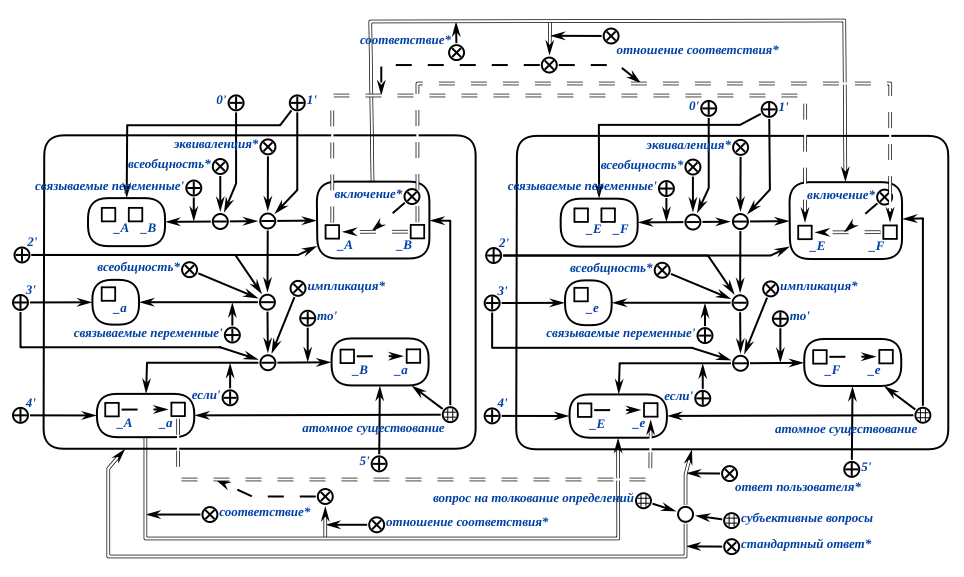
\includegraphics[scale=0.65]{author/part7/figures/establishment_mapping_relationship_example.png}
	\caption{Пример установления отношений отображения потенциальных эквивалентных пар переменных sc-узлов между семантическими графами}
	\label{fig:EMR_example}
\end{figure}

Поэтому, на основе подхода к преобразованию формул логики предикатов в ПНФ и некоторых характеристик логических формул в ostis-системах, в данной подглаве предлагается подход к преобразованию логических формул в уникальные (детерминированные) ПНФ в соответствии со строгими правилами ограничения. Строгие правила ограничения в основном включают следующее:

\begin{itemize}
	\item чтобы решить проблему, заключающуюся в том, что ПНФ не являются уникальными из-за порядка использования различных формул логической эквивалентности, мы указываем, что правило переименования должно использоваться предпочтительно при преобразовании логических формул в ПНФ;
	
	\item для решения проблемы, что ПНФ не является уникальной из-за порядка кванторов, в данной подглаве предлагается подход, позволяющий перемещать все кванторы в передний конец логической формулы строго в соответствии с приоритетом кванторов. Процесс перемещения кванторов показан ниже:
	
	\begin{itemize}
		\item если в начале логической формулы не существует кванторов, то все кванторы существования перемещаются в начало логической формулы по преимуществу;
		
		\item если последний квантор в переднем конце логической формулы является квантором всеобщности, то кванторы всеобщности в логической формуле будут преимущественно перемещены в начало формулы;
		
		\item если последний квантор в переднем конце логической формулы является квантором существования, то кванторы существования в логической формуле будут перемещены преимущественно в начало формулы.
	\end{itemize}
	
	\item логическая формула, используемая для представления ответа на вопрос на толкование определений, обычно может быть выражена в следующей форме: ($Q_{1}x_{1}Q_{2}x_{2}\cdots Q_{n}x_{n}(A\leftrightarrow B)$), где $Q_{i}\left ( i = 1, \cdots n \right )$ представляет собой квантор [\scncite{Li2021a}], [\scncite{Krom1970}]. $A$ используется для описания определения понятия на целостном уровне, и кванторы в него не включены. $B$ используется для объяснения семантического оттенка определения на уровне детализации, и обычно эта формула является логической формулой, содержащей кванторы (также известной как логическая подформула). Поэтому, исходя из характеристик логической формулы и для упрощения обработки знаний, необходимо лишь преобразовать логическую формулу $B$ в ПНФ;
	
	\item для упрощения обработки знаний при преобразовании логических формул в ПНФ необходимо исключить только связку импликации;
	
	\item несколько атомарных логических формул, соединённых с помощью одной и той же связки конъюнкции, предпочтительно объединяются в одно целое (т.е. они объединяются в одну sc-структуру).
	
\end{itemize}

Процесс преобразования семантических графов ответов на вопросы на толкование определений в описание ПНФ в соответствии со строгими правилами ограничения показан ниже:

\begin{itemize}
	\item если в семантическом графе имеется несколько sc-структур, соединённых одной и той же связкой конъюнкции, то содержащиеся в них sc-конструкции объединяются в одну sc-структуру;
	
	\item исключение всех связок импликации в семантических графах;
	
	\item перемещение всех связок отрицания в семантических графах в передний конец соответствующей sc-структуры;
	
	\item использование правила переименования, чтобы все связанные переменные в семантических графах не были одинаковыми;
	
	\item перемещение всех кванторов в первый конец логической формулы;
	
	\item снова объединение sc-структур, которые могут быть объединены в семантическом графе.
	
\end{itemize}

Пример преобразования логической формулы в ПНФ показан на рисунке (\textit{\nameref{fig:PNF_example}}) в SCg-коде ($\forall A\forall B((A\subseteq B) \leftrightarrow \forall a(a\in A\rightarrow a\in B))$ $\Leftrightarrow$ $\forall A\forall B((A\subseteq B) \leftrightarrow \forall a ( \neg ( a\in A ) \lor (a\in B)))$).

\begin{figure}[H]
	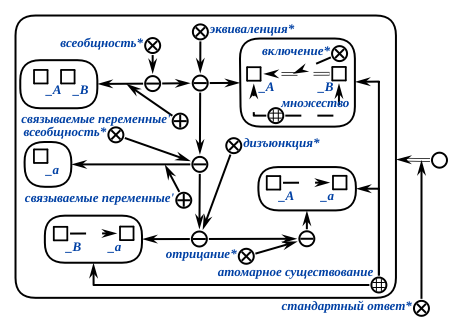
\includegraphics[scale=0.8]{author/part7/figures/PNF_example.png}
	\caption{Пример преобразования семантического графа в представление ПНФ}
	\label{fig:PNF_example}
\end{figure}

Следует подчеркнуть, что если вычисленное подобие между семантическими графами представления ПНФ не равно 1 ($F_{sc}$ < 1), то в качестве окончательного подобия ответа используется подобие между семантическими графами, вычисленное в первый раз. Когда подобие между ответами получено, а затем объединено со стратегией оценки субъективных вопросов, можно проверить правильность и полноту ответов пользователей [\scncite{Li2021a}].

~\\
\textbf{Вычисление подобия между ответами на вопросы на доказательство и на решение задачи} 

~\\
Как вопросы на доказательство, так и решение задачи в математике следуют общему процессу решения задач:

\begin{enumerate}
	\item набор условий ($\Omega $), состоящий из некоторых известных условий;
	
	\item выведение промежуточного вывода с использованием некоторых известных условий в $\Omega $ и добавление его к $\Omega $. Каждый элемент в $\Omega $ можно рассматривать как шаг решения;
	
	\item повторять шаг 2 до получения окончательного результата [\scncite{Zhang1995}], [\scncite{Zhang2019}].
\end{enumerate}

Этот процесс решения задачи абстрагируется в виде направленного графа, структура которого в большинстве случаев представляет собой перевернутое дерево (в особых случаях направленный граф будет содержать цикл), (рисунок \textit{\nameref{fig:RT_example}}), и называется деревом рассуждений (т.е. деревом рассуждений стандартного ответа).

\begin{figure}[H]
	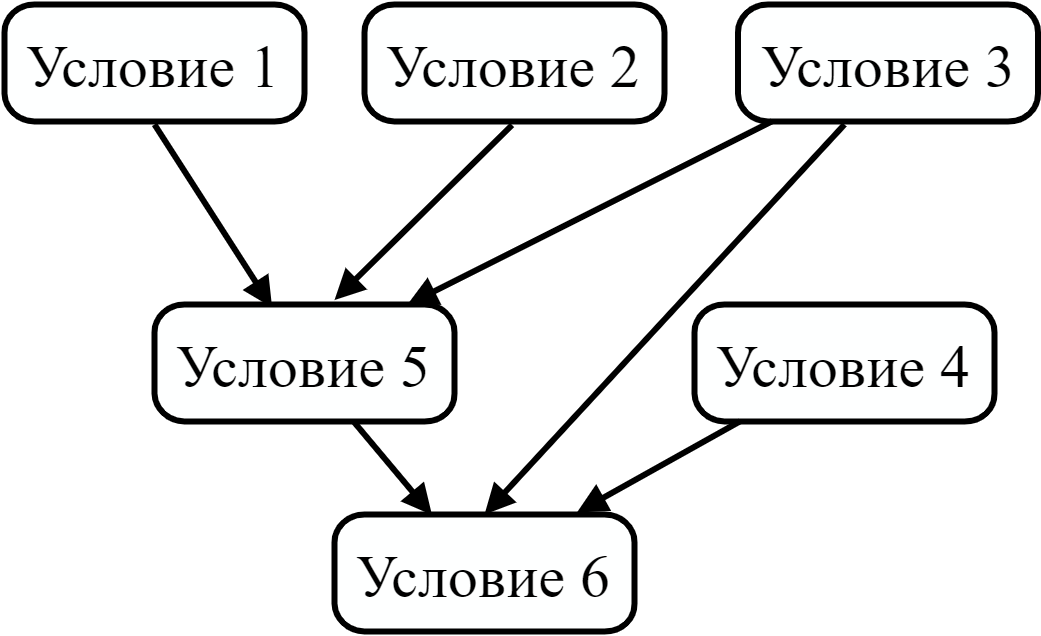
\includegraphics[scale=0.15]{author/part7/figures/reasoning_tree_example.png}
	\caption{Пример дерева рассуждений}
	\label{fig:RT_example}
\end{figure}

Ответ пользователя на вопрос на доказательство или на решение задачи представляет собой линейную структуру, состоящую из некоторых шагов решения (т.е. известных условий, промежуточных условий или выводов), каждый из которых удовлетворяет строгим отношениям выведения и логическим отношениям, если ответ пользователя полностью правильный. Процесс автоматической проверки ответов пользователя на данный тип тестовых вопросов аналогичен традиционной ручной проверке ответов, т.е. проверка того, является ли текущий шаг решения ответа пользователя правильным заключением частичного шага решения, предшествующего этому шагу. Это означает, всегда ли шаг решения в ответе пользователя, соответствующий родительскому узлу в дереве рассуждений, располагается после шагов решения в ответе пользователя, соответствующих дочерним узлам.

Семантические графы ответов пользователя на вопросы на доказательство и на решение задачи в ostis-системах представляют собой линейные структуры, состоящие из некоторых семантических подграфов для описания шагов решения и некоторых семантических фрагментов для описания логического порядка и процессов преобразования между семантическими подграфами [\scncite{Golenkov2014b}], [\scncite{IMS}]. Процесс построения и семантическая спецификация семантических графов ответов пользователя на вопросы на доказательство и на решение задачи подробно описаны в работе [\scncite{Shunkevich2015}]. Семантические графы стандартных ответов на тестовые вопросы такого типа представляют собой деревья рассуждений, состоящие из некоторых шаблонов поиска (которые могут абстрагироваться как узлы в дереве). Каждый шаблон поиска построен строго в соответствии со стандартными шагами решения соответствующего тестового вопроса (т.е. в соответствии с известными условиями, промежуточными условиями и выводами в $\Omega $). Шаблон поиска в ostis-системах используется для поиска в базе знаний всех соответствующих ему семантических фрагментов, и он построен на основе SCL-кода. Далее в качестве примера взято реальное решение задачи, чтобы представить построение его семантического графа ответа пользователя (рисунок \textit{\nameref{fig:STE_example}}) и семантического графа стандартного ответа (дерева рассуждений), (рисунок \textit{\nameref{fig:ITE_example}}). Описание решения задачи: <<Две равные окружности внешне касаются другой и третьей окружности, радиус которой равен 4. Отрезок, торой соединяет точки касания двух равных окружностей с третьей, равен 6. Найдите радиусы равных окружностей.>>, (рисунок \textit{\nameref{fig:EI_example}}). 

\begin{figure}[H]
	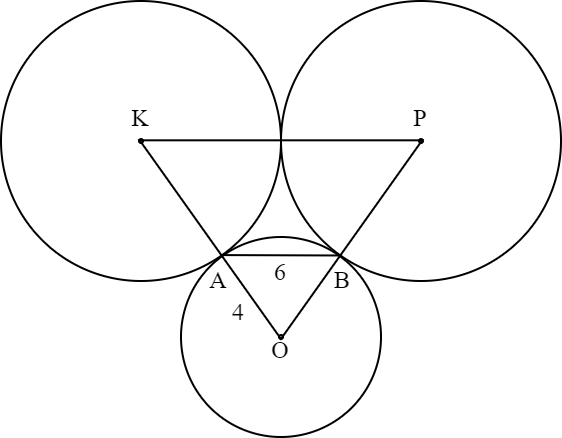
\includegraphics[scale=0.3]{author/part7/figures/explanatory_illustration_example.png}
	\caption{Пояснительный рисунок к решению задачи}
	\label{fig:EI_example}
\end{figure}

Описание ответа пользователя на естественном языке:

\begin{enumerate}
	\item $\because KP = 2*R$
	\item $\because KO = 4+R$
	\item $\therefore \Delta A O B\backsim \Delta K O P$
	\item $\therefore K A = R = 12$
\end{enumerate}

Ответы пользователей на естественном языке преобразуются в семантические графы с помощью естественно-языковых интерфейсов. Поэтому при вычислении подобия между семантическими графами ответов нет необходимости учитывать различия понятий на уровне естественного языка [\scncite{Qian2020a}]. Пример спецификации конкретного понятия показан на рисунке (\textit{\nameref{fig:SSE_example}}).

\begin{figure}[H]
	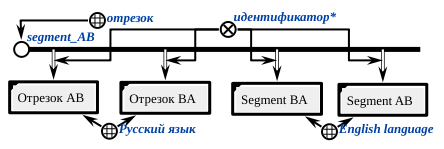
\includegraphics[scale=0.8]{author/part7/figures/specification_segment_example.png}
	\caption{Пример семантической спецификации отрезка AB}
	\label{fig:SSE_example}
\end{figure}

\begin{figure}[H]
	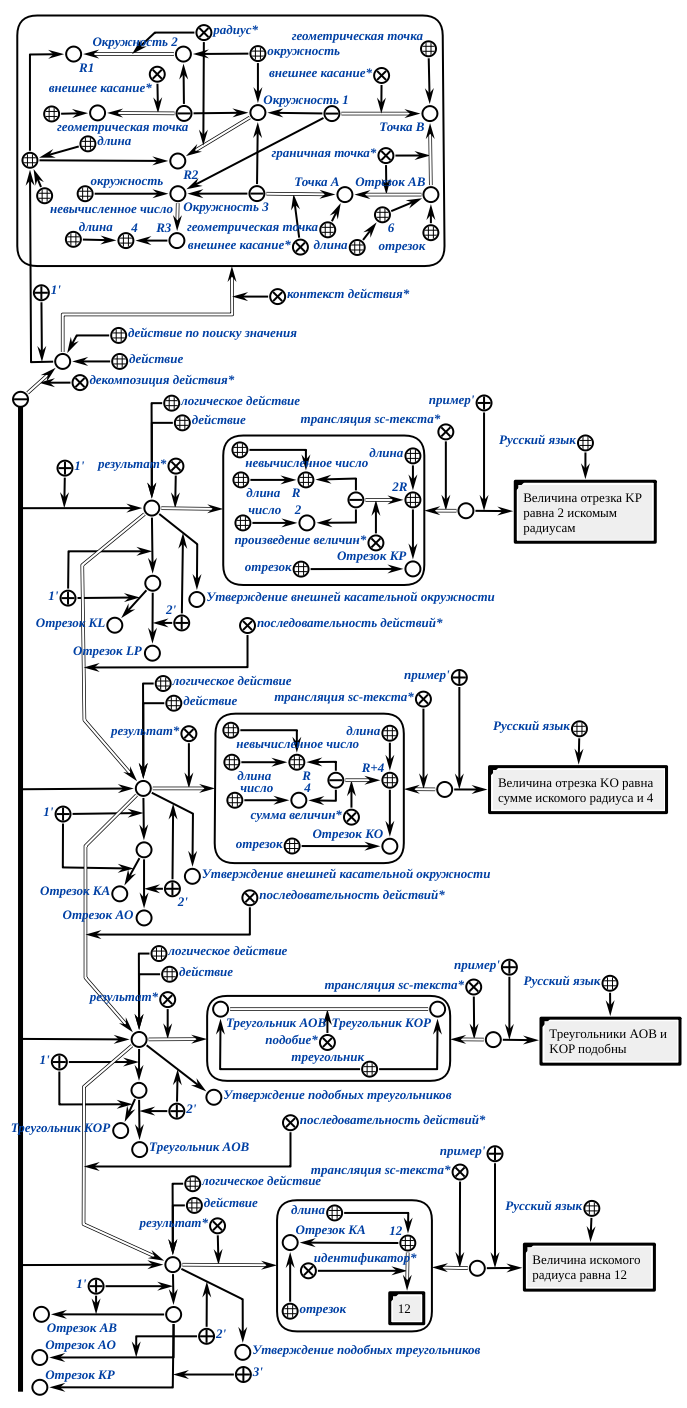
\includegraphics[scale=0.7]{author/part7/figures/solving_task_example.png}
	\caption{Пример семантической модели ответа пользователя на решение задачи}
	\label{fig:STE_example}
\end{figure}

\begin{figure}[H]
	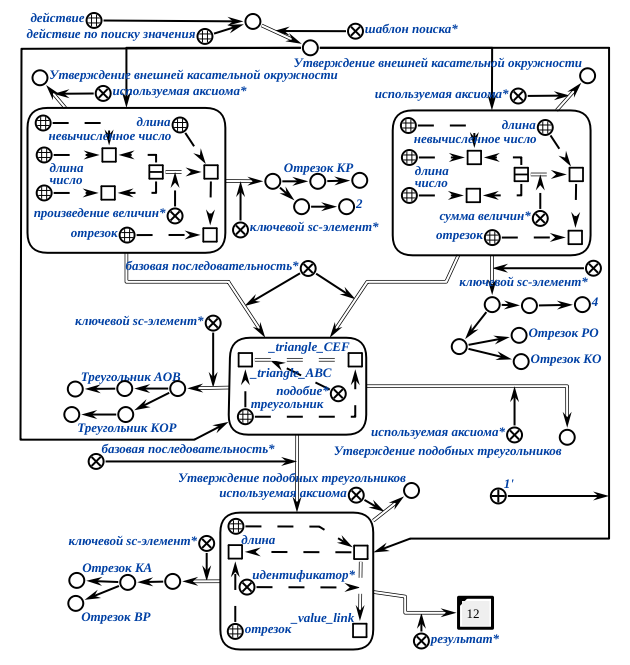
\includegraphics[scale=0.6]{author/part7/figures/inference_tree_example_SCg.png}
	\caption{Пример семантической модели дерева рассуждений стандартного ответа}
	\label{fig:ITE_example}
\end{figure}

Из рисунка (\textit{\nameref{fig:SSE_example}}) видно, что Отрезок AB и Отрезок BA представлены одним и тем же sc-узлом, они просто являются двумя идентификаторами sc-узла. Поэтому на основе ранее представленного принципа автоматической проверки ответов пользователя на вопросы на доказательство и на решение задачи и семантических моделей ответов в ostis-системах, в данной подглаве предлагается подход к вычислению подобия между семантическими графами ответов на вопросы на доказательство и на решение задачи в соответствии с деревом рассуждений стандартного ответа (семантический граф стандартного ответа). Процесс вычисления подобия между семантическими графами показан ниже:

\begin{enumerate}
	\item нумерация каждого семантического подграфа (шага решения) в семантическом графе ответов пользователей (порядок нумерации начинается с 1);
	
	\item каждый узел (шаблон поиска) в дереве рассуждений обходится по очереди в соответствии со стратегией DFS. В то же время, соответствующий семантический подграф, включенный в семантический граф ответа пользователя, ищется в базе знаний с использованием шаблона поиска, который обходится в данный момент. Если такой семантический подграф существует, то определить, меньше ли нумерация найденного семантического подграфа, чем нумерация семантического подграфа, соответствующего шаблону поиска родительского узла текущего шаблона поиска (кроме корневого узла дерева рассуждений), и если да, то найденный семантический подграф считается правильным;
	
	\item повторять шаг 2, пока не будут обойдены все шаблоны поиска в дереве рассуждений и одновременно подсчитано количество правильных семантических подграфов;
	
	\item использование формул (\ref{formula_7_5_1}), (\ref{formula_7_5_2}) и (\ref{formula_7_5_3}) для вычисления точности $P_{sc}$, полноты $R_{sc}$ и подобия $F_{sc}$ между ответами. Параметры в формуле переопределены:
	
	\begin{itemize}
		\item $|T_s{_c}(u)|$ --- количество всех семантических подграфов в семантическом графе ответа пользователя $u$; 
		\item $|T_s{_c}(s)|$ --- количество всех шаблонов поиска в дереве рассуждений $s$; 
		\item $|T_s{_c}(u)\otimes T_s{_c}(s)|$ --- количество правильных семантических подграфов.
	\end{itemize}
	
\end{enumerate}

После получения подобия между ответами на вопросы на доказательство и на решение задачи, правильность и полнота ответов пользователей может быть проверена в сочетании со стратегией оценки субъективных вопросов.

Стратегия оценки субъективных вопросов показана ниже:

\begin{itemize}
	\item если подобие между ответами равно 1 ($F_{sc}$ = 1), то ответ пользователя полностью правильный и пользователь получает максимальный балл ($Max_{score}$);
	
	\item если подобие между ответами меньше 1 ($F_{sc}$ < 1) и точность равна 1 ($P_{sc}$ = 1), то ответ пользователя правильный, но неполный, и оценка пользователя равна $R_{sc}*Max_{score}$;
	
	\item если подобие между ответами больше 0 и меньше 1, а точность меньше 1 (0 < $F_{sc}$ < 1 и $P_{sc}$ < 1), то ответ пользователя является частично правильным и оценка пользователя равна $P_{sc}*Max_{score}$;
	
	\item если подобие между ответами равно 0 ($F_{sc}$ = 0), то ответ пользователя является неправильным и оценка пользователя равна 0 [\scncite{Li2021a}].
\end{itemize}

Предлагаемый подход к автоматической проверке ответов пользователей имеет следующие преимущества:

\begin{itemize}
	\item проверка правильности и полноты ответов пользователя на основе семантики;
	
	\item можно проверить правильность и полноту ответов пользователя на любые типы тестовых вопросов и определить логическую эквивалентность между ответами;
	
	\item позволяет вычислять подобие между любыми двумя семантическими графами в базе знаний;
	
	\item предложенный подход может быть использован в различных ostis-системах.
\end{itemize}

\subsection{Семантическая модель базы знаний подсистемы}

База знаний подсистемы в основном используется для хранения автоматически сгенерированных тестовых вопросов различных типов, а также позволяет автоматически извлекать ряд тестовых вопросов и формировать экзаменационные билеты в соответствии с требованиями пользователя. Поэтому для повышения эффективности доступа к базе знаний подсистемы и эффективности извлечения тестовых вопросов в данной подглаве предлагается подход к построению базы знаний подсистемы в соответствии с типом тестовых вопросов и стратегией генерации тестовых вопросов. Основой базы знаний любой ostis-системы (точнее, sc-моделью базы знаний) является иерархическая система предметных областей и соответствующих им онтологий [\scncite{Golenkov2014b}], [\scncite{Shunkevich2015}], [\scncite{IMS}]. Рассмотрим иерархию базы знаний подсистемы в SCn-коде:

\scnheader{Раздел. Предметная область тестовых вопросов}

\begin{scnreltoset}{декомпозиция раздела}
	
	\scnitem{Раздел. Предметная область субъективных вопросов}
	
	\begin{scnreltoset}{декомпозиция раздела}
		\scnitem{Раздел. Предметная область вопроса на толкование определений}
		\scnitem{Раздел. Предметная область вопроса на доказательство}
		\scnitem{Раздел. Предметная область решения задачи}
	\end{scnreltoset}
	
	\scnitem{Раздел. Предметная область объективных вопросов}
	
	\begin{scnreltoset}{декомпозиция раздела}
		\scnitem{Раздел. Предметная область вопроса на выбор}
		\scnitem{Раздел. Предметная область вопроса на заполнение пробелов}
		\scnitem{Раздел. Предметная область вопроса суждения}
	\end{scnreltoset}
	
\end{scnreltoset}

Далее, взяв в качестве примера предметную область объектных вопросов, рассмотрим ее структурную спецификацию в SCn-коде:

\scnheader{Предметная область объективных вопросов}
\scniselement{предметная область}
\scnhaselementrole{максимальный класс объектов исследования}{объективный вопрос}
\begin{scnhaselementrolelist}{немаксимальный класс объектов исследования}
	\scnitem{вопрос на выбор}
	\scnitem{вопрос на заполнение пробелов}
	\scnitem{вопрос суждения} 
\end{scnhaselementrolelist}

Объективные типы тестовых вопросов могут быть разложены на более конкретные типы в соответствии с их характеристиками и соответствующими стратегиями генерации тестовых вопросов. Далее, взяв в качестве примера вопрос на выбор, рассмотрим его семантическую спецификацию в SCn-коде:

\scnheader{вопрос на выбор}
\scniselementrole{максимальный класс объектов исследования}{Предметная область вопроса на выбор}

\begin{scnreltoset}{разбиение}
	
	\scnitem{вопрос на выбор на основе свойств отношений}
	\scnitem{вопрос на выбор на основе идентификаторов}
	\scnitem{вопрос на выбор на основе примеров изображения}
	\scnitem{вопрос на выбор на основе аксиом}
	\scnitem{вопрос на выбор на основе элементов}
	
	\begin{scnreltoset}{разбиение}
		\scnitem{вопрос на выбор на основе бинарного отношения}
		\scnitem{вопрос на выбор на основе ролевого отношения}
	\end{scnreltoset}
	
	\scnitem{вопрос на выбор на основе классов}
	
	\begin{scnreltoset}{разбиение}
		\scnitem{вопрос на выбор на основе отношения разбиения}
		\scnitem{вопрос на выбор на основе отношения строгого включения}
		\scnitem{вопрос на выбор на основе отношения включения}
	\end{scnreltoset}
	
\end{scnreltoset}

\begin{scnreltoset}{разбиение}
	\scnitem{вопрос на выбор с несколькими вариантами ответа}
	\scnitem{вопрос на выбор с одним вариантом ответа}
\end{scnreltoset}

\begin{scnreltoset}{разбиение}
	\scnitem{выбор неправильного варианта}
	\scnitem{выбор правильного варианта}
\end{scnreltoset}


\subsection{Семантическая модель решателя задач}

Решатель задач любой ostis-системы (точнее, sc-модель решателя задач ostis-системы) представляет собой иерархическую систему агентов обработки знаний в семантической памяти (sc-агенты), которые взаимодействуют только путем указания действий, выполняемых ими в указанной памяти [\scncite{Golenkov2014b}].

Поэтому для решения соответствующих задач в данной подглаве разработан решатель задач для автоматической генерации тестовых вопросов и автоматической проверки ответов пользователей, иерархия которого представлена следующим образом в SCn-коде:

\scnheader{Решатель задач для автоматической генерации тестовых вопросов и автоматической проверки ответов пользователей}

\begin{scnreltoset}{декомпозиция абстрактного sc-агента}
	
	\scnitem{Sc-агент для автоматической генерации тестовых вопросов}
	
	\begin{scnreltoset}{декомпозиция абстрактного sc-агента}
		\scnitem{Sc-агент для быстрой генерации тестовых вопросов и экзаменационных билетов}
		\scnitem{Sc-агент для генерации тестовых вопросов одного типа}
		\scnitem{Sc-агент для генерации единого экзаменационного билета}
	\end{scnreltoset}
	
	\scnitem{Sc-агент для автоматической проверки ответов пользователей}
	
	\begin{scnreltoset}{декомпозиция абстрактного sc-агента}
		\scnitem{Sc-агент для автоматической оценки экзаменационных билетов}
		\scnitem{Sc-агент для вычисления подобия между ответами на объективные вопросы}
		\scnitem{Sc-агент для оценки логической эквивалентности между семантическими графами, описанными на основе фактических знаний}
		\scnitem{Sc-агент для вычисления подобия между ответами на вопросы на толкование определений}
		\scnitem{Sc-агент для преобразования логической формулы в ПНФ}
		\scnitem{Sc-агент для вычисления подобия между ответами на решение задачи и на вопросы на доказательство}
	\end{scnreltoset}
	
\end{scnreltoset}

Основная функция sc-агента для быстрой генерации тестовых вопросов и экзаменационных билетов заключается в автоматизации всего процесса от генерации тестовых вопросов до генерации экзаменационных билетов путём инициирования соответствующих sc-агентов (sc-агент для генерации тестовых вопросов одного типа и sc-агент для генерации единого экзаменационного билета). Основной функцией sc-агента для генерации тестовых вопросов одного типа является автоматическая генерация ряда тестовых вопросов из базы знаний с использованием логических правил, построенных на основе SC-кода [\scncite{IMS}]. Логические правила для генерации тестовых вопросов построены строго в соответствии со стратегиями генерации тестовых вопросов, описанными ранее. Пример логического правила приведён на рисунке (\textit{\nameref{fig:LRE_example}}).

\begin{figure}[H]
	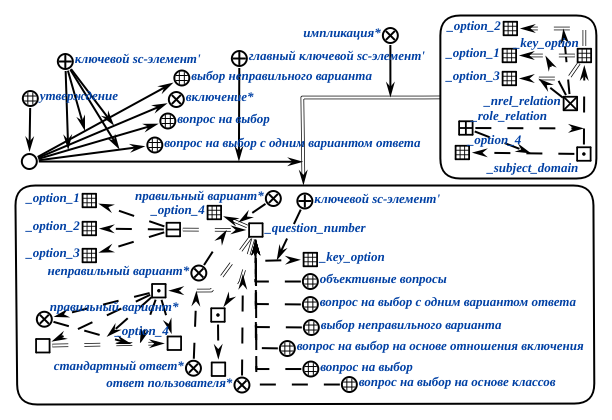
\includegraphics[scale=1]{author/part7/figures/logic_rule_example.png}
	\caption{Пример логического правила для генерации вопроса на выбор}
	\label{fig:LRE_example}
\end{figure}

Основная функция sc-агента для автоматической оценки экзаменационных билетов заключается в реализации автоматической проверки ответов пользователей на различные типы тестовых вопросов и автоматической оценки экзаменационных билетов путём инициирования sc-агентов для вычисления подобия между ответами пользователей, sc-агента для оценки логической эквивалентности между семантическими графами, описанными на основе фактических знаний и sc-агента для преобразования логической формулы в ПНФ.

\subsection{Оценка эффективности подсистемы}

Далее мы оценим эффективность разработанной подсистемы с точки зрения удобства использования сгенерированных тестовых вопросов, сложности сформированных тестовых билетов и близости между результатами ручной оценки и автоматической оценки ответов пользователей на тестовые вопросы.

Для того чтобы оценить удобство использования тестовых вопросов, автоматически сгенерированных с помощью базы знаний, из обучающей системы по дискретной математике были случайным образом выбраны 200 автоматически сгенерированных тестовых вопросов, соответственно, в соответствии с типом тестового вопроса и соответствующей пропорцией, и пропорция тестовых вопросов, которые могут быть использованы напрямую, была подсчитана ручным методом (\textit{\nameref{tab:usability_test_questions}}).

\begin{table}[!htbp]
	\centering
	\caption{Таблица. Результаты оценки удобства использования сгенерированных тестовых вопросов по дискретной математике}
	\label{tab:usability_test_questions}
	%\scalebox{0.95}
	%{	
		\begin{tabular}{|p{0.2\textwidth}|p{0.25\textwidth}|p{0.3\textwidth}|p{0.2\textwidth}|} 
			\hline 
			Показатели доступности&Тестовые вопросы,  которые можно использовать напрямую&Тестовые вопросы, которые могут быть использованы после внесения изменений&Недоступные тестовые вопросы\\
			\hline  
			Количество тестовых вопросов (всего 200)&188&12&0\\
			\hline
			Пропорция&94\%&6\%&0\\
			\hline  
		\end{tabular}
		%}	
\end{table}

Из таблицы (\textit{\nameref{tab:usability_test_questions}}) видно, что среди 200 случайно выбранных тестовых вопросов по дискретной математике, 94\% тестовых вопросов могут быть использованы  напрямую, а 6\% тестовых вопросов могут быть использованы после внесения изменений.

Сложность экзаменационных билетов тесно связана с распределением баллов пользователей. Таким образом, далее мы случайным образом выберем 40 студентов 2-го курса, чтобы оценить сложность экзаменационного билета по дискретной математике, сгенерированного случайным образом с помощью подсистемы. В экзаменационный билет включены 10 вопросов на выбор, 10 вопросов на заполнение пробелов, 10 вопросов суждения, 2 вопроса на толкование определений и 2 вопроса на доказательство. Максимальный балл за каждый объективный вопрос составляет 2 балла, максимальный балл за каждый субъективный вопрос составляет 10 баллов, а максимальный балл за весь экзаменационный билет составляет 100 баллов (\textit{\nameref{tab:score_exam_paper}}). 

\begin{table}[!htbp]
	\centering
	\caption{Таблица. Статистические результаты оценки студентов}
	\label{tab:score_exam_paper}
	%\scalebox{0.95}
	%{	
		\begin{tabular}{|p{0.1\textwidth}|p{0.12\textwidth}|p{0.12\textwidth}|p{0.12\textwidth}|p{0.12\textwidth}|p{0.12\textwidth}|p{0.12\textwidth}|p{0.12\textwidth}|} 
			\hline 
			Балл& <40 & [40-49] & [50-59] & [60-69] & [70-79] & [80-89] & >=90 \\
			\hline  
			Количество студентов всего 40) & 0 & 1 & 4 & 10 & 14 & 8 &3 \\
			\hline
			Пропорция & 0 & 2.5\% & 10\% & 25\% & 35\% & 20\% & 7.5\% \\
			\hline
			Средний балл & \multicolumn{7}{c|}{72.85} \\
			\hline  
		\end{tabular}
		%}	
\end{table}

Как видно из таблицы (\textit{\nameref{tab:score_exam_paper}}), результаты тестов студентов в основном подчиняются нормальному распределению. Таким образом, можно сделать вывод, что  сложность текущего типа экзаменационного билета является умеренной, и фактический уровень знаний и ситуация обучения пользователей могут быть проверены объективно и беспристрастно.

Для того чтобы оценить близость между результатами ручной оценки и автоматической оценки ответов пользователей на субъективные вопросы, мы решили сначала ввести в соответствующую систему ответы 40 студентов на субъективные вопросы в экзаменационном билете по дискретной математике, затем использовать подсистему для автоматической проверки ответов студентов и, наконец, подсчитать ошибку между результатами автоматической оценки и ручной оценки ответов пользователей на субъективные вопросы (\textit{\nameref{tab:error_statistics_result}}). .

\begin{table}[!htbp]
	\centering
	\caption{Таблица. Результаты статистики ошибок оценки за ответы пользователей на субъективные вопросы}
	\label{tab:error_statistics_result}
	%\scalebox{0.95}
	%{	
		\begin{tabular}{|p{0.14\textwidth}|p{0.14\textwidth}|p{0.14\textwidth}|p{0.14\textwidth}|p{0.14\textwidth}|p{0.12\textwidth}|p{0.12\textwidth}|} 
			\hline 
			Диапазон ошибок ($\Phi $) & Вопрос на  толкование  определений 1 & Вопрос на  толкование  определений 2 & Вопрос на  доказательство 1 & Вопрос на  доказательство 2 & Итог & Пропорция \\
			\hline  
			$\Phi$<=1 & 35 & 31 & 26 & 28 & 120 & 75\% \\
			\hline
			(1-1.5] & 2 & 4 & 8 & 8 & 22 & 13.75\% \\
			\hline
			(1.5-2] & 2 & 3 & 5 & 3 & 13 & 8.125\% \\
			\hline
			$\Phi$>2 & 1 & 2 & 1 & 1 & 5 & 3.125\% \\
			\hline
		\end{tabular}
		%}	
\end{table}

Процесс вычисления ошибки $\Phi $ приведён в формуле (\ref{formula_7_6_4}):

\begin{equation}    
	\Phi =\sqrt{\left ( x -y \right ) ^{2} }   
	\label{formula_7_6_4} 
\end{equation}

Где $x$ --- ручная оценка ответа пользователя на соответствующий тестовый вопрос, и $y$ --- автоматическая оценка ответа пользователя на соответствующий тестовый вопрос.

Из таблицы (\textit{\nameref{tab:error_statistics_result}}) видно, что в обучающей системе по дискретной математике результаты ручной оценки и результаты автоматической оценки ответов пользователей на субъективные вопросы в основном согласуются, и когда максимальная оценка за субъективные вопросы составляет 10 баллов, размер выборки с ошибкой $\Phi$ <= 1.5 между результатами ручной оценки и результатами автоматической оценки составляет более 88\%.

Из приведенных выше результатов эксперимента видно, что разработанная подсистема может удовлетворять условиям практического применения.

\subsection{Заключение}

В этой подглаве предлагается основанный на семантике подход к автоматической генерации тестовых вопросов и автоматической проверке ответов пользователей в ostis-системах. На основе предложенного подхода разработана универсальная подсистема для автоматической генерации тестовых вопросов и автоматической проверки ответов пользователей. Разработанная подсистема позволяет автоматизировать весь процесс от генерации тестовых вопросов до оценки экзаменационных билетов.

Основным принципом автоматической генерации тестовых вопросов является автоматическая генерация объективных и субъективных вопросов из базы знаний с использованием некоторых правил, построенных на основе структурных особенностей базы знаний ostis-систем. Основной принцип автоматической проверки ответов пользователей заключается в том, чтобы сначала вычислить подобие между семантическими графами ответов, а затем объединить его со стратегией оценки соответствующего тестового вопроса для реализации автоматической проверки ответов пользователей (включая суждение о логической эквивалентности между ответами). Предложенный подход к вычислению подобия между ответами также позволяет вычислять подобие между любыми двумя семантическими графами в базе знаний, поэтому в будущем данный подход может быть использован для решения других задач (таких как отображение онтологий, слияние знаний и т.д.). Наконец, из результата оценки эффективности подсистемы видно, что разработанная подсистема может соответствовать условиям практического применения.


\section{Дидактические знания}
\label{section_knowledge_control}

%\input{author/references}